\subsubsection{\theoryC{High mass diboson resonance search at HE-LHC}}
\contributors{C. Helsens, D. Jamin, M. Selvaggi}\rt{There are comments to address.}
%{\bf Authors: C. Helsens$^1$, D. Jamin$^2$, M. Selvaggi$^3$}\\
%\newline
%$^1$CERN EP-Departement, CH-1211 Geneva 23, Switzerland email: {\tt B.C. clement.helsens@cern.ch}\\
%$^2$Academia Sinica, Institute of  Physics, Taipei, Taiwan\\


%\newcommand*{\zptt}{\ensuremath{Z^{\prime} \rightarrow \ttbar}}
%\newcommand*{\qjj}{\ensuremath{Q^{*} \rightarrow jj}}
%\newcommand*{\rsg}{\ensuremath{G_{RS} \rightarrow WW}}
%\newcommand*{\vj}{\ensuremath{\text{V + jets}}}
%\newcommand*{\metvec}{\vec{\pt}^{\textrm{miss}}}
%\newcommand*{\intlumihelhc}{\ensuremath{\mathcal{L}=15\text{ ab}^{-1}}}

%\textbf{Reponsible: Clement Helsens, Michele Selvaggi}

%%%%%%%%%%%%%%%%%%%%%%%%%%%%%%%%%%%%%%%%%%%%%%%%%%%%%%%%%%%%%%%%%%%%%%%%%%%%%%%%%%%%%%%%%%%%
%\subsubsection{Introduction}
%\paragraph*{Introduction}
%Many models of beyond the SM (BSM) physics predict additional particles with masses at the TeV scale. 
The presence of new resonant states~\cite{Harris:2011bh,Boelaert:2009jm,Lee:1973iz,Branco:2011iw,Hill:1994hp,Kaplan:1983sm,Bellazzini:2014yua,Randall:1999ee,Pomarol:1999ad} decaying to two highly boosted particles decaying hadronically could be observed at the LHC as an excess over the SM dijet invariant mass distribution. We focus here on the specific benchmark model: Randall-Sundrum graviton~\cite{Randall:1999ee}. We study the sensitivity in the following decay using hadronic $G_{RS} \rightarrow WW$\ decay mode.

The decay product is typically in the multi-TeV regime and its reconstruction imposes stringent requirement on the detector design. Precise jet energy resolution requires full longitudinal shower containment. Highly boosted $W$ bosons decay into highly collimated jets that need to  be disentangled from standard QCD jets by studying their substructure. High discrimination power and sensitivity for this search at such extreme energies, requires excellent granularity both in the tracking detectors and calorimeters. \rt{Some text is equal to the $t\bar{t}$ section from the same authors. It should be fixed.}

%%%%%%%%%%%%%%%%%%%%%%%%%%%%%%%%%%%%%%%%%%%%%%%%%%%%%%%%%%%%%%%%%%%%%%%%%%%%%%%%%%%%%%%%%%%%
%\subsubsection{Monte Carlo Samples}
%\paragraph*{Monte Carlo Samples}
Signal events were generated at LO with \pythia~8.230~\cite{Sjostrand:2014zea}. The SM backgrounds are dijet (QCD), top pairs ($\ttbar$), $VV$ and $V+\text{ jets}$\ where $V=W/Z$, which were generated using \MGvATNLO 2.5.2~\cite{Alwall:2014hca} at LO. A k-factor of 2 is applied to all the background processes.\rt{As in the other contributions this thing makes little sense to me.}

%%%%%%%%%%%%%%%%%%%%%%%%%%%%%%%%%%%%%%%%%%%%%%%%%%%%%%%%%%%%%%%%%%%%%%%%%%%%%%%%%%%%%%%%%%%%
%\subsubsection{Multivariate tagger}
%\paragraph*{Multivariate tagger}
\label{sec:mvatagger2}
An important ingredient of the $G_{RS} \rightarrow WW$\ search is the identification of heavy boosted $W$ bosons. A jet tagger using Boosted Decision Trees (BDTs) was developed to discriminate $W$ jets against the $\pt$ dijet background.
%NB: Need to define if more material needed.

%Top and $W$ taggers were optimised using jets with a transverse boost of $\pt=$10 TeV. At these extreme energies, $W$ and top jets have a characteristic angular size $R=0.01-0.02$, i.e smaller than the typical electromagnetic and hadronic calorimeter cells. Following the approach described in \citeref{Larkoski:2015yqa}, we exploit the superior track angular resolution and reconstruct jets from tracks only (track jets) using the anti-$k_T$ algorithm with a parameter R=0.2. The missing neutral energy is corrected for by rescaling the track 4-momenta by the factor $\ptSup{trk}/\ptSup{PF}$, where $\ptSup{trk}$ is the track Jet \pt\ and $\ptSup{PF}$ is the Particle-Flow Jet \pT. In what follows, we will simply refer to ``track jets'' as the jet collection that includes the aforementioned rescaling.
%
%The boosted top tagger is built from jet substructure observables: the soft-dropped jet mass~\cite{Larkoski:2014wba} and N-subjettiness~\cite{Thaler:2010tr} variables $\tau_{1,2,3}$ and their ratios $\tau_{2}/\tau_{1}$ and $\tau_{3}/\tau_{2}$. The $W$-jet versus QCD-jet tagger also uses an ``isolation-like'' variable that exploits the absence of high \pt\ final state-radiation (FSR) in the vicinity of the $W$ decay products. We call these variables $E_{F}(n,\alpha)$ and define them as:
%
%\begin{equation}
%E_{F}(n,\alpha) =  \frac{\sum \limits_{\frac{n-1}{5}\alpha < \Delta R(k,jet)< \frac{n}{5}\alpha} \ptSup{(k)}}{\sum \limits_{\Delta R(k,jet)< \alpha} \ptSup{(k)}}
%\end{equation}
%
%We use $\alpha=0.05$. We construct 5 variables $E_{F}(n,\alpha)$ with $n=1..5$ and provide them as input to the BDT. The $E_{F}(1,0.05)$ observable is shown in \fig{fig:hadronicresonances:BDTeff} (left).
%The final performance of the $W$ and top tagger is shown in \fig{fig:hadronicresonances:BDTeff} (right). The $W$ tagging performance has significantly better performance due to the use of the energy-flow variables. We choose our working points with a top and $W$ tagging efficiencies of $\epsilon_S^{\text{top}}=60\%$ and $\epsilon_S^{\text{W}}=90\%$ corresponding respectively to a background efficiency of $\epsilon_B^{\text{top}}=\epsilon_B^{\text{W}}=10\%$.
%
%
%\begin{Figure}
%  \centering
%  \includegraphics[width=0.37\columnwidth]{\main/img/hadronicresonances/Jet1_Flow15_sel0_nostack_logx.eps}
%  \includegraphics[width=0.45\columnwidth]{\main/img/hadronicresonances/effQCD_vs_effWhadBlue_thadRed_log.eps}
%  \caption{Left: Energy-flow ($E_{F}(1,0.05)$) observable for W and QCD jets. Right: Dijet rejection versus signal efficiency for the two taggers, W in blue and top in red.%\MS{need editing - REDO left EFlow in logX - Right: need legend and stars}
%  }
%  \label{fig:hadronicresonances:BDTeff}
%\end{Figure}

%%%%%%%%%%%%%%%%%%%%%%%%%%%%%%%%%%%%%%%%%%%%%%%%%%%%%%%%%%%%%%%%%%%%%%%%%%%%%%%%%%%%%%%%%%%%
%\subsubsection{Event Selection}
%\paragraph*{Event Selection}
As track jets are better able to resolve the jet sub-structure compared to particle-flow jets, the jet selection for the $G_{RS} \rightarrow WW$\ search is using track jets. As no lepton veto is applied, there is also some acceptance for leptonic decays. The sensitivity to semi-leptonic $WW$ decays is enhanced by adding the $\vec{\pt}^{\textrm{miss}}$ vector to the closest jet 4-momentum (among the to leading jets).

We require two jets with a $\pt$>1~TeV and $|\eta|<3$ and $\Delta(\eta)<2.4$. Both jets must be $W$ tagged. Finally, to further reject QCD, we require for both jets $m_{SD}>40$~GeV. In left \fig{fig:hadronicresonances:wwsel04} we show the dijet invariant mass distribution after the final analysis cuts.

%%%%%%%%%%%%%%%%%%%%%%%%%%%%%%%%%%%%%%%%%%%%%%%%%%%%%%%%%%%%%%%%%%%%%%%%%%%%%%%%%%%%%%%%%%%%
%\subsubsection{Signal extraction and results}
%\paragraph*{Signal extraction and results}
Hypothesis testing is performed using a modified frequentist method based on a profile likelihood fit that takes into account the systematic uncertainties as nuisance parameters. The dijet invariant mass is used as a discriminant. In order to reduce large statistical fluctuations from high Monte Carlo weight events, we parameterize the background invariant mass distribution with the following function (conservatively assuming 50\% uncertainty on the background normalisation) $f(z)=p_1(1-z)^{p_2}z^{p_3}z^{p_{4}logz}$, where $z=m_{jj}/\sqrt{s}$.

The expected exclusion limit at 95\%~\cl and discovery reach at $5 \sigma$ are shown in middle and right Figures~\ref{fig:hadronicresonances:wwsel04}. Reconstructing Heavy resonances decaying to $WW$ is challenging and requires the use of novel approaches to boosted object tagging to reduce the backgrounds. The reach for $G_{RS} \rightarrow WW$\ model is $\sim8$ TeV and it is possible to discover it up to $m_{RSW}\sim$ 7 TeV.

\begin{figure}[htbp]
  \centering
  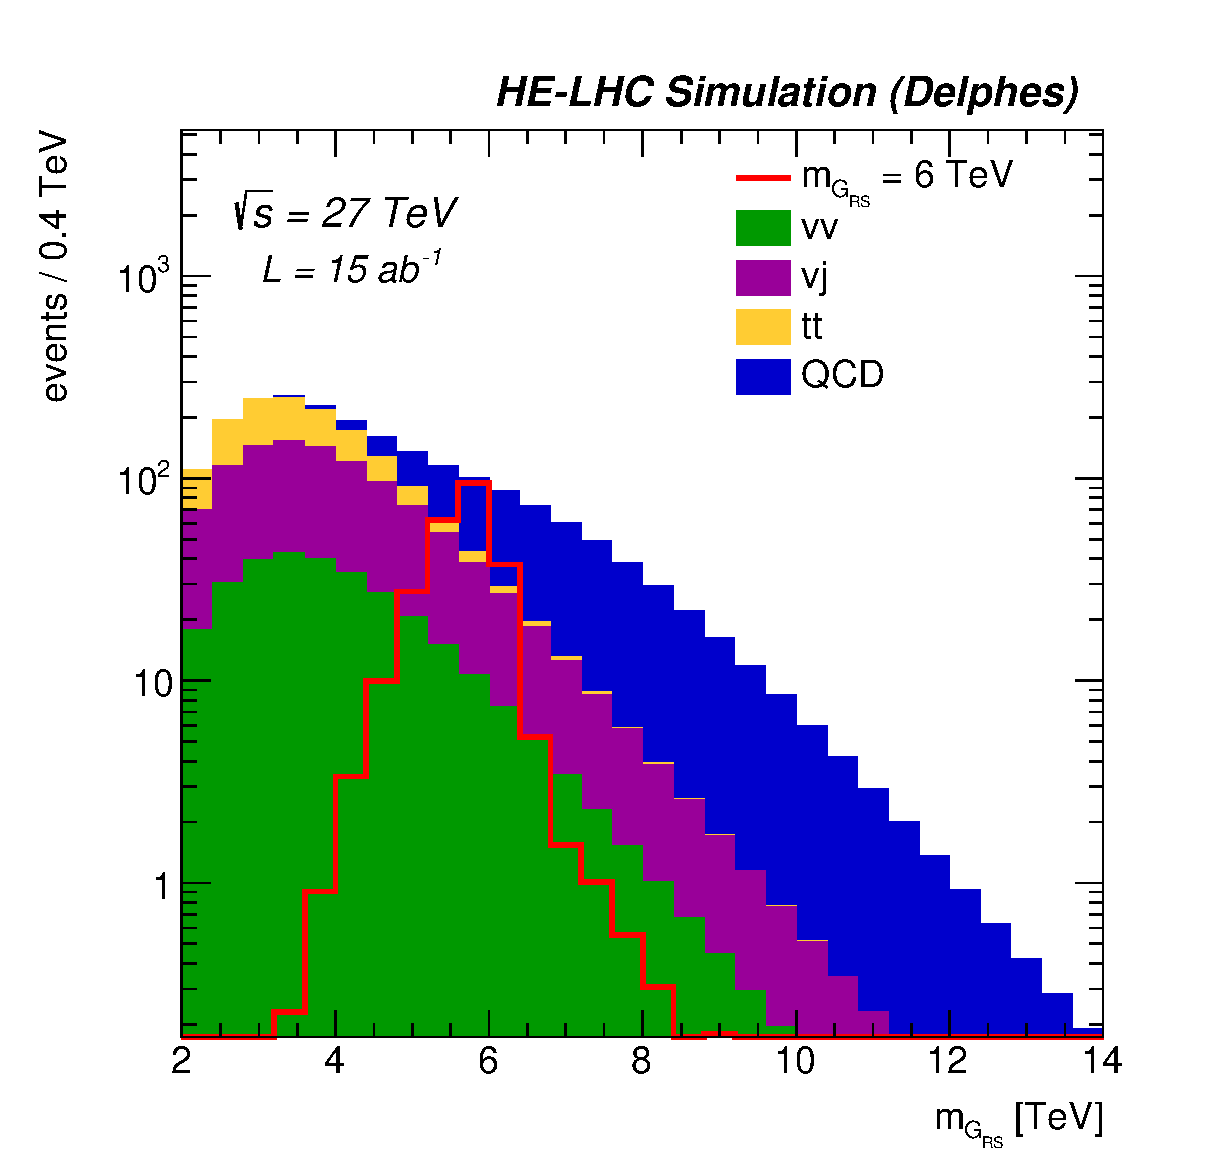
\includegraphics[width=0.30\columnwidth]{\main/section7OtherSignatures/img/RSGWW_Mj1j2_pf08_fit_sel4_nostack_log.eps}
  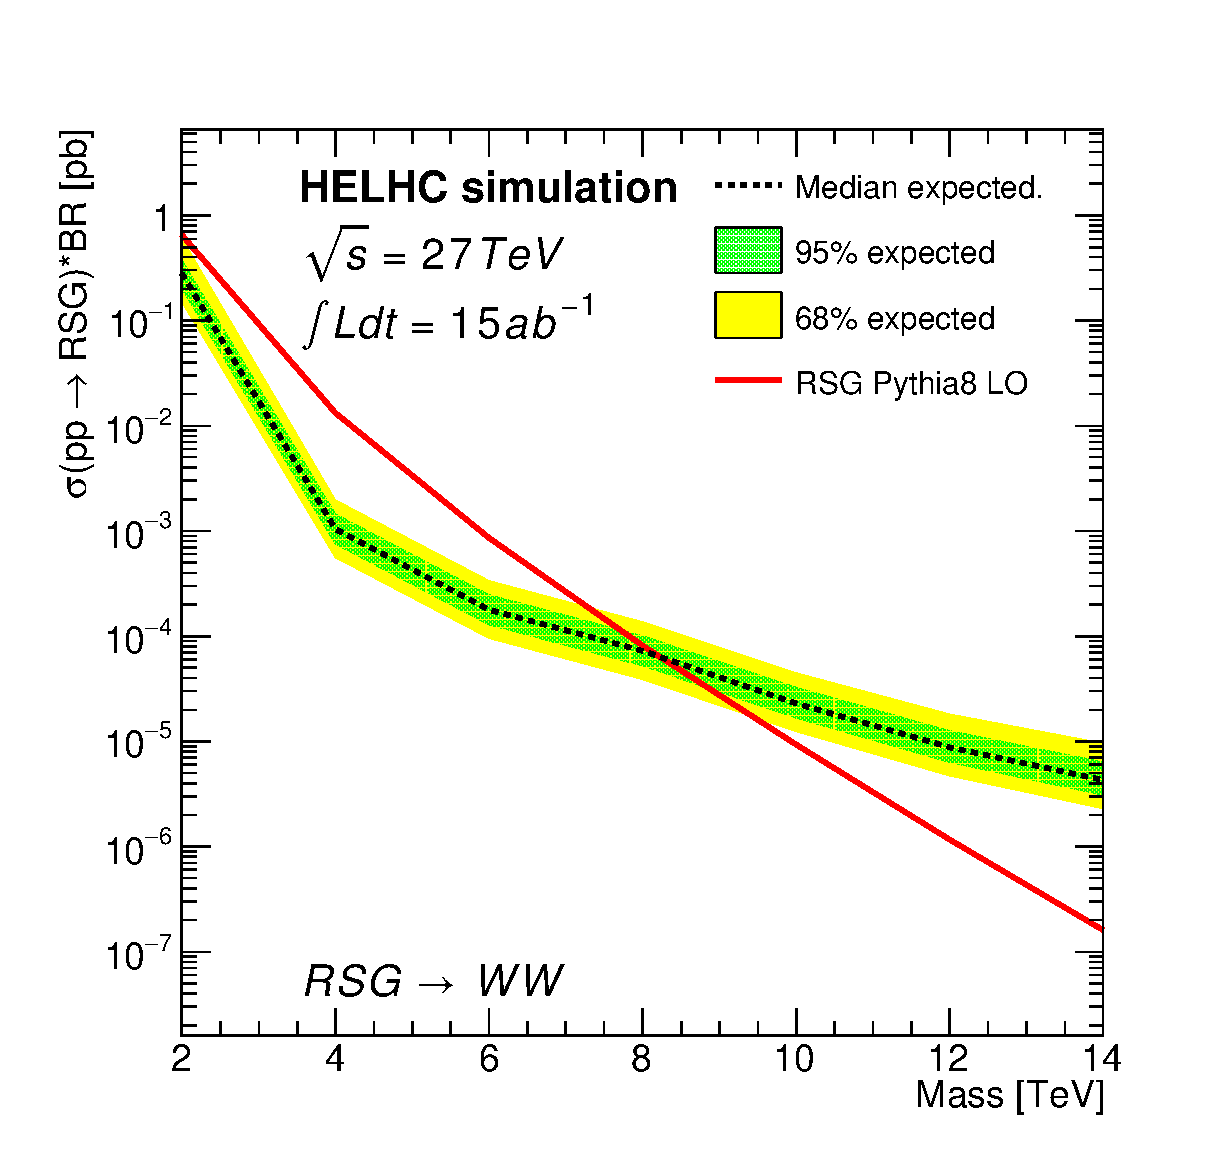
\includegraphics[width=0.30\columnwidth]{\main/section7OtherSignatures/img/lim_RSGraviton_ww_helhc_v01.eps}
  \includegraphics[width=0.30\columnwidth]{\main/section7OtherSignatures/img/DiscoveryPotential_ww_tagger_rootStyle.eps}

  \caption{Left distribution : invariant mass distribution of the two leading jets for the full selection for a 6~TeV signal for the $G_{RS} \rightarrow WW$\ analysis. Middle distribution : exclusion limit at 95\%~\cl versus heavy resonance mass. Right distribution : integrated luminosity for a $5\sigma$ discovery as a function of the heavy resonance mass.}
  \label{fig:hadronicresonances:wwsel04}
\end{figure}

\begin{table}[!htb]\centering
\scalebox{0.9}{
\begin{tabular}{|c|c|c|}
\hline
\hline
signal $m_{RSG}$= & 2 TeV  &  284.6 \\
                  & 4 TeV  &  789.7 \\
                  & 6 TeV  &  245.7 \\
                  & 8 TeV  &   49.0 \\
                  & 10 TeV &    8.7 \\
                  & 12 TeV &    1.4 \\
                  & 14 TeV &    0.8 \\
\hline
background        & vv     &  302.3 \\
                  & vj     &  794.4 \\
                  & tt     &  516.3 \\
                  & QCD    &  547.7 \\
                  & total  & 2160.7 \\
\hline
\hline
\end{tabular}}
\caption{Final yield of $RSG \rightarrow WW$ analysis.}
\label{tab:RSGwwYield}
\end{table}


